\documentclass[12pt, a4paper]{ntut-report}
\usepackage[dvips,xetex]{graphicx}
\usepackage{ifpdf,mla}% <-- mla.sty requires ifpdf.sty, but (perversely) doesn't load it
%\usepackage{fontspec}
\usepackage{geometry}
\usepackage{lipsum}
\usepackage{xeCJK}
\usepackage{wallpaper}
\usepackage{pdfpages}
\usepackage{indentfirst}
\usepackage{setspace}
\usepackage{hyperref}
\usepackage{zhnumber}
\usepackage{titlesec}
\usepackage{amsmath}
\usepackage[backend=bibtex,sorting=none]{biblatex}   

\renewcommand{\baselinestretch}{1.5}
\xeCJKsetup{AutoFakeBold=true, AutoFakeSlant=true}
\setCJKmainfont{標楷體} % 中文字體
\setmainfont{Times New Roman} % 英文字體
\geometry{a4paper,total={297mm,210mm},top=4.5cm,bottom=0.75cm,left=2.5cm,right=2.5cm} % 頁面設定,不需修改
\pagestyle{plain} % 頁碼
\addbibresource{reference.bib}

%
% this file is encoded in utf-8
%

%% 這些設定值將會用於呈現在首頁上,請進行填入
%% Please fill in the information which will be shown on the cover and in the abstract. All Chinese and English information must be matched to each other. If you don’t have any Chinese information, please skip the Chinese ones, but all English Information is required.

%
% 中文論文設定值,請根據以下的範例進行填入
%

% 論文題目(中文)
% Thesis Title (Chinese)
\newcommand\cTitle{基於沙盒系統之程式評測應用}

% 我的姓名(中文)
% My Name(Chinese)
\newcommand\myCname{黃漢軒}

% 指導教授的姓名 (中文),使用頓號隔開 
% Advisor (Chinese), use “、” to separate names
\newcommand\advisorCname{郭忠義 博士}

% 校名 (中文)
% School Name(Chinese)
\newcommand\univCname{國立臺北科技大學}

% 系所名 (中文)
% Department Name(Chinese)
\newcommand\deptCname{資訊工程系碩士班}

% 學位名 (中文)
% Degree Name(Chinese)
\newcommand\degreeCname{碩士}

% 口試年份 (中文、民國)
% Year of Oral Defense(Chinese)
\newcommand\cYear{一百一十二}

% 口試月份 (中文)
% Month of Oral Defense(Chinese)
\newcommand\cMonth{七} 

% 畢業學年度 (中文)
% 如 112 學年度第2學期畢業,當時為民國113年6月,學年度即為112,不是113。
\newcommand\cAcademicYear{一百一十二}

% 畢業學期(中文)
% Academic Year (Chinese)
\newcommand\cGraduateSemester{二}

%
% 英文論文設定值,請根據以下的範例進行填入
%

% 論文題目 (英文)
% Thesis Title (Engslih)
\newcommand\eTitle{Online Judge System based on Sandbox System}

% 我的姓名(英文)
% My Name(English)
\newcommand\myEname{Huang, Han-Xuan}

% 指導教授的姓名 (英文),使用逗號隔開
% 例如:Dr. Kuo Jong-Yi, Dr. A B-C, ...
%
% Advisor (Ensligh), use “, ” to separate names
% e.g. Dr. Kuo Jong-Yi, Dr. A B-C, ...
\newcommand\advisorEname{Dr. Kuo Jong-Yi}

% 校名(英文)
% School Name(English)
\newcommand\univEname{National Taipei University of Technology}

% 系所全名 (英文)
% Department Name(English)
\newcommand\fulldeptEname{Department of Computer Science and Information Engineering}

\newcommand\deptEname{Computer Science and Information Engineering}

% 學位名 (英文)
% Degree(English)
\newcommand\degreeEname{Master of Science}

% 口試年份 (阿拉伯數字、西元)
% Year of Oral Defense(English)
\newcommand\eYear{2023}

% 口試月份 (英文)
% Month of Oral Defense(English)
\newcommand\eMonth{June}

%畢業級別;用於書背列印;若無此需要可忽略
\newcommand\GraduationClass{111}

%%%%%%%%%%%%%%%%%%%%%%

\begin{document}

% 封面、不用浮水印 Cover without a watermark
\begin{titlepage}
    \newpage
    \begin{center}
        % NTUT logo
        
\includegraphics[width=13cm]{ntut-logo-with-label.png}
        
        \huge\bf\fulldeptEname \\% Department's name
        \huge\bf\degreeEname\\ % “Master Thesis” or “Ph.D. Dissertation”

        \vfill
        \LARGE\bf\eTitle\\ %%%%%

        \vfill
        {\Large Researcher: \myEname}

        \vfill
        {\Large Advisor: \advisorEname}

        \vfill
        {\Large \eMonth, \eYear}
    \end{center}
\end{titlepage}
% 留白頁、不用浮水印 Blank page without a watermark
\newpage
\thispagestyle{empty}

% 新增浮水印 Add Watermarks
\CenterWallPaper{.64}{ntut-logo.png}

% 封面、要浮水印 Cover with a watermark
\begin{titlepage}
    \newpage
    \begin{center}
        % NTUT logo
        
\includegraphics[width=13cm]{ntut-logo-with-label.png}
        
        \huge\bf\fulldeptEname \\% Department's name
        \huge\bf\degreeEname\\ % “Master Thesis” or “Ph.D. Dissertation”

        \vfill
        \LARGE\bf\eTitle\\ %%%%%

        \vfill
        {\Large Researcher: \myEname}

        \vfill
        {\Large Advisor: \advisorEname}

        \vfill
        {\Large \eMonth, \eYear}
    \end{center}
\end{titlepage}
% 「學位論文口試委員會審定書」掃描檔,請檢附完整簽名之審定書掃描檔
% Please add "Oral Defense Committee Signature Form" with complete signatures.
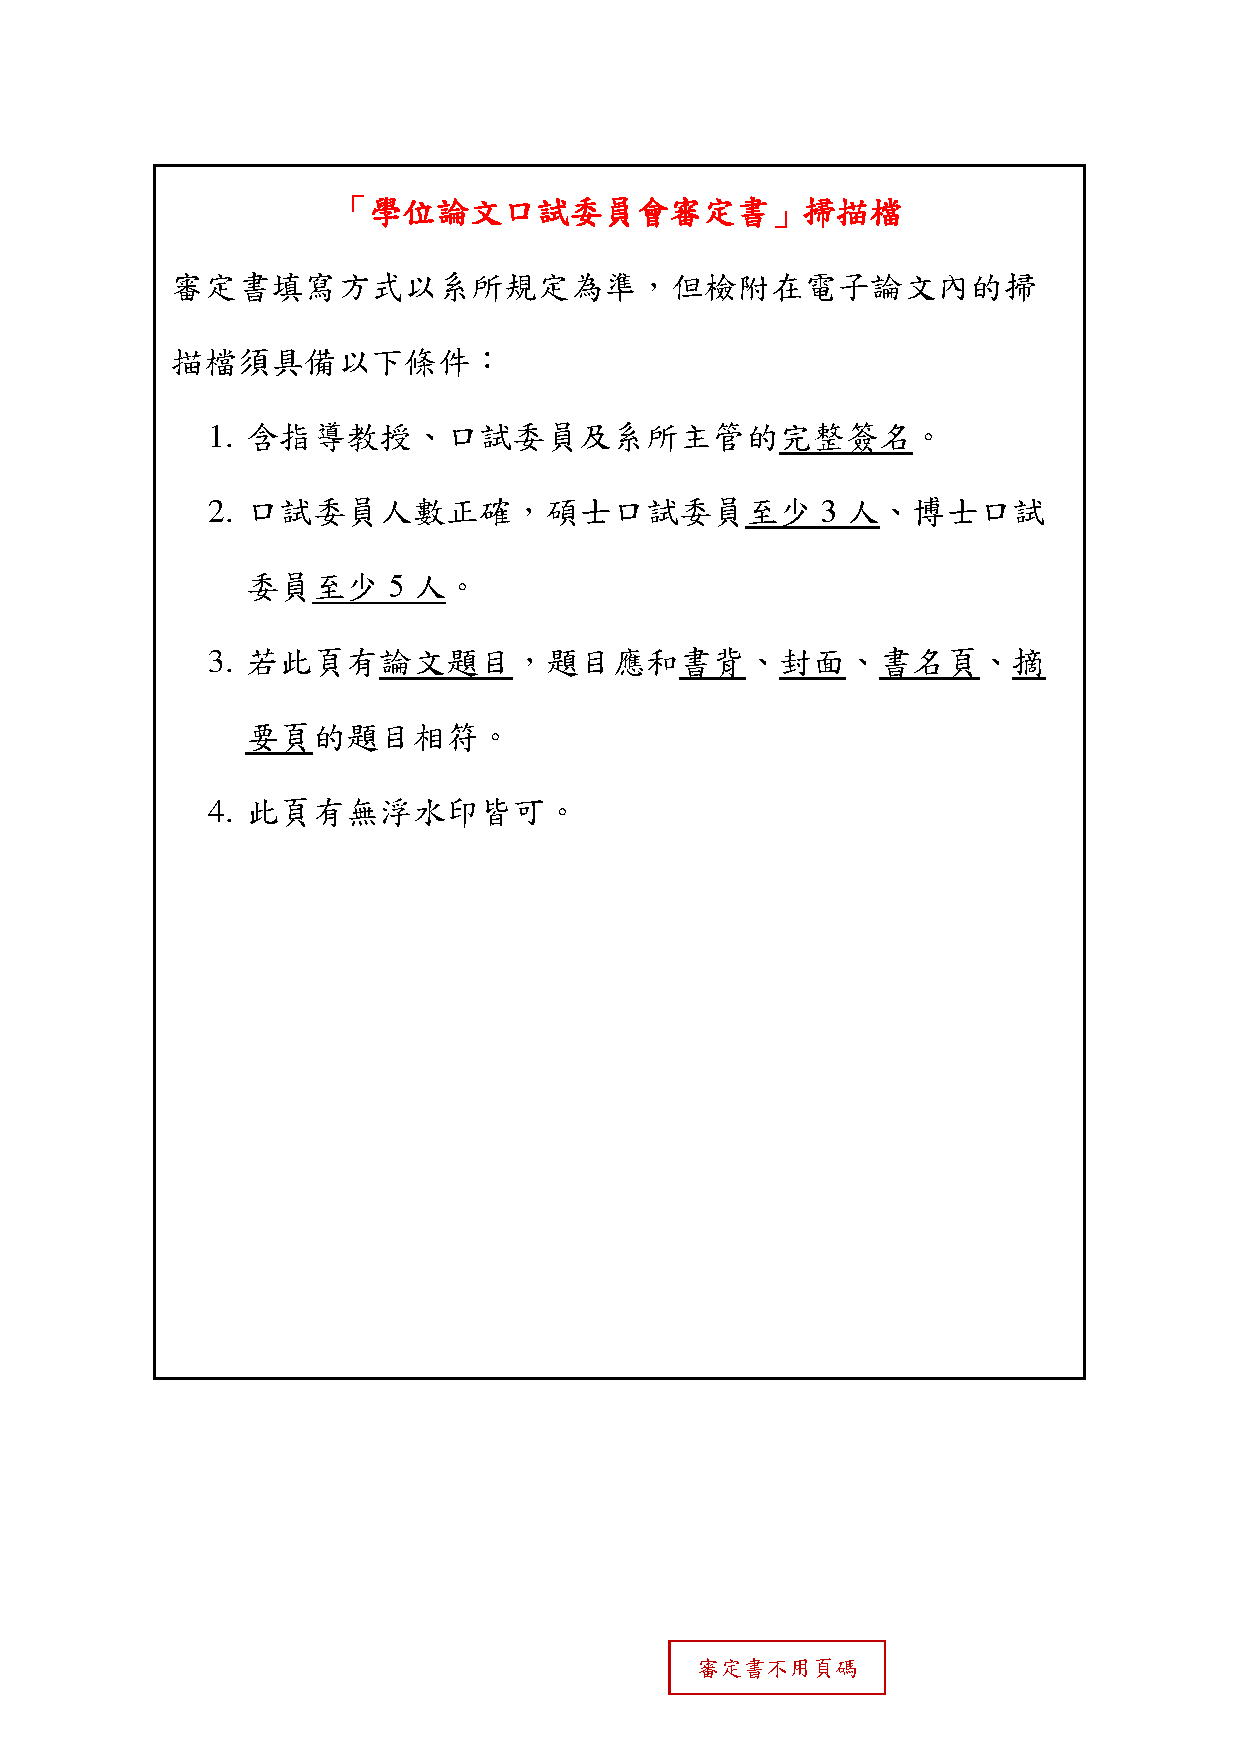
\includepdf[pages=-]{static-page/signpage.pdf}

\pagenumbering{roman}

% 摘要頁(中文)Abstract (Chinese)
% If you don’t have Chinese abstract, please delete this one.
% 中文摘要頁
\begin{ZhAbstract}
    \begin{ZhAbstractItems}
        % 論文名稱,請在 ntut-labels.tex 定義
        \noindent \text 論文名稱:\cTitle

        % 論文頁碼,請在 ntut-labels.tex 定義
        \noindent \text 頁碼:(請自己填)

        % 校所別,請在 ntut-labels.tex 定義
        \noindent \text 校所別:\univCname \space \deptCname

        % 畢業時間,請在 ntut-labels.tex 定義
        \noindent \text 畢業時間:\cYear 學年度 \space 第\cGraduateSemester 學期

        % 學位,請在 ntut-labels.tex 定義
        \noindent \text 學位:\degreeCname

        % 研究生,請在 ntut-labels.tex 定義
        \noindent \text 研究生:\myCname

        % 指導教授,請在 ntut-labels.tex 定義
        \noindent \text 指導教授:\advisorCname

        % 關鍵詞,請自己填
        \noindent \text 關鍵詞:(請自己填)

    \end{ZhAbstractItems}

    \begin{ZhAbstractDescription}
        摘要為論文或報告的精簡概要,其目的是透過簡短的敘述使讀者大致瞭解整篇報告的內容。摘要的內容通常須包括問題的描述以及所得到的結果,但以不超過 500 字或一頁為原則,且不得有參考文獻或引用圖表等。以中文撰寫之論文除中文摘要外,得於中文摘要後另附英文摘要。標題使用 20pt 粗標楷體並於上、下方各空一行(1.5 倍行高,字型 12pt 空行)後鍵入摘要內容。摘要頁須編頁碼(小寫羅馬數字表示頁碼)。
    \end{ZhAbstractDescription}
    
\end{ZhAbstract}


% 摘要頁(英文)Abstract (English)
% 英文摘要頁
\begin{EnAbstract}
    \begin{EnAbstractItems}
        % 論文名稱,請在 ntut-labels.tex 定義
        \noindent \text Title: \eTitle

        % 論文總頁數,同最後一頁阿拉伯數字頁碼
        % Page number, same as the page number of the last page, not the total pages in pdf file.
        \noindent \text Pages: (Fill it)

        % 校所別,請在 ntut-labels.tex 定義
        \noindent \text School: \univEname

        % 系所別,請在 ntut-labels.tex 定義
        \noindent \text Department: \deptEname

        % 畢業時間,請在 ntut-labels.tex 定義
        \noindent \text Time: \eMonth, \eYear

        % 學位,請在 ntut-labels.tex 定義
        \noindent \text Degree: \degreeEname

        % 研究生,請在 ntut-labels.tex 定義
        \noindent \text Researcher: \myEname

        % 指導教授,請在 ntut-labels.tex 定義
        \noindent \text Advisor: \advisorEname
        
        % 關鍵詞,請自己填,多個關鍵字以逗號 "," 隔開
        \noindent \text Keyword: (Fill it)

    \end{EnAbstractItems}

    \begin{EnAbstractDescription}
        Start writing abstract from here. Start writing abstract from here. Start writing abstract from here. Start writing abstract from here. Start writing abstract from here. Start writing abstract from here. Start writing abstract from here. Start writing abstract from here.
    \end{EnAbstractDescription}
    
\end{EnAbstract}


% 鳴謝 Acknowledgements
\begin{Thanks}
    所有對於研究提供協助之人或機構,作者都可在誌謝中表達感謝之意。
\end{Thanks}
% 目錄、表目錄與圖目錄 Table of Contents, List of tables, List of figures
\begin{TableOfContent}
    \tableofcontents
\end{TableOfContent}

\begin{TableOfContent}
    \listoftables
\end{TableOfContent}

\begin{TableOfContent}
    \listoffigures
\end{TableOfContent}
 
\pagenumbering{arabic}

% 章節一 Chapter 1
\begin{ZhChapter}

\chapter{緒論(大標)}

\section{研究動機與背景(小標)}

\begin{equation} 
    \mbox{$x = \dfrac{-b\pm\sqrt{b^2-4ac}}{2a}$}
\end{equation}

\subsection{研究背景(小小標)}

\text 背景內文背景內文背景內文背景內文,背景內文背景內文背景內文背景內文背景內文背景內文,如表 1.1 所示。

\begin{table*}[htbp]
    \centering
    \caption{表格範例標題} \label{tab: complexity}
    \makebox[\linewidth][c]{
    \renewcommand\arraystretch{1.2}{
        \begin{tabular}{| l | c  c  c  c |}
        \hline
        Protocol & $P$ & $CS_1$ & $CS_2$ & $RG$ \\
        \hline
        SD & $O(1)$, $O(1)$, N/A & $O(n-t)$, $O(1)$, N/A & $O(n-t)$, $O(1)$, N/A & $O(1)$, $O(n)$, $O(n)$ \\
        MSSMul & $O(1)$, $O(1)$, N/A & $O(n-t)$, $O(n)$, $O(1)$ & $O(n-t)$, $O(n)$, N/A & $O(1)$, $O(n)$, $O(n)$ \\
        MSSAdd & $O(1)$, $O(1)$, N/A & $O(n-t)$, $O(n)$, $O(1)$ & N/A, N/A, N/A & $O(1)$, $O(n)$, $O(n)$ \\
        SC & $O(1)$, $O(1)$, N/A & $O(n-t)$, $O(n)$, $O(1)$ & $O(n-t)$, $O(n)$, N/A & $O(1)$, $O(n)$, $O(n)$ \\
        \hline 
        \end {tabular}
    }}
\end {table*}

\subsubsection{研究動機(小小標)}

\begin{equation} 
    \mbox{$(1+x)^n = 1 + \dfrac{nx}{1!} + \dfrac{n(n-1)x^2}{2!}$}
\end{equation}

動機動機動機動機,動機動機動機動機動機動機動機動機動機動機動機動機,動機動機動機動機動機動機動機動機。

動機動機動機動機動機動機動機動機,動機動機動機動機動機動機動機動機動機動機動機動機。動機動機動機動機動機動機動機動機,動機動機動機動機動機動機動機動機動機動機動機動機。動機動機動機動機動機動機動機動機,動機動機動機動機動機動機動機動機動機動機動機動機,如圖 1.1、圖 1.2 所示。

\begin{figure*}[htbp]
    \centering
    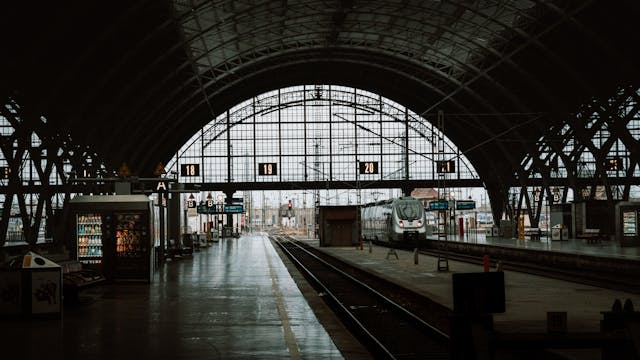
\includegraphics[width = 1\textwidth]{image.jpeg}
    \caption{Cool train station}
    \label{fig: image}
\end{figure*}

\begin{figure*}[htbp]
    \centering
    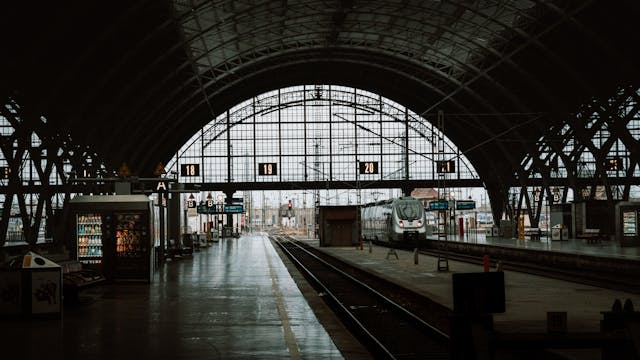
\includegraphics[width = 1\textwidth]{image.jpeg}
    \caption{"Cool train station" "Cool train station" "Cool train station" "Cool train station" "Cool train station" "Cool train station" "Cool train station" "Cool train station" "Cool train station" "Cool train station" "Cool train station" "Cool train station"}
    \label{fig: image}
\end{figure*}

\begin{figure*}[htbp]
    \centering
    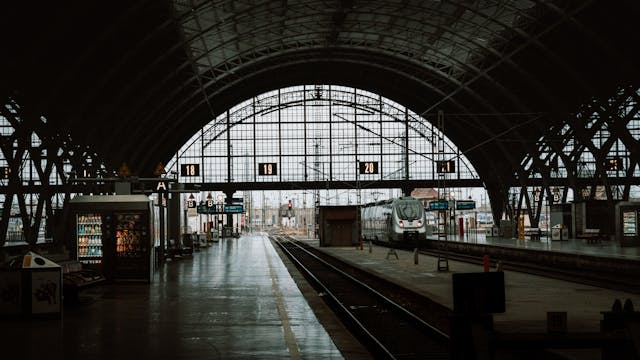
\includegraphics[width = 1\textwidth]{image.jpeg}
    \caption{Cool train station}
    \label{fig: image}
\end{figure*}

\begin{table*}[htbp]
    \centering
    \caption{表格範例標題} \label{tab: complexity}
    \makebox[\linewidth][c]{
    \renewcommand\arraystretch{1.2}{
        \begin{tabular}{| l | c  c  c  c |}
        \hline
        Protocol & $P$ & $CS_1$ & $CS_2$ & $RG$ \\
        \hline
        MSSMul & $O(1)$, $O(1)$, N/A & $O(n-t)$, $O(n)$, $O(1)$ & $O(n-t)$, $O(n)$, N/A & $O(1)$, $O(n)$, $O(n)$ \\
        MSSAdd & $O(1)$, $O(1)$, N/A & $O(n-t)$, $O(n)$, $O(1)$ & N/A, N/A, N/A & $O(1)$, $O(n)$, $O(n)$ \\
        SC & $O(1)$, $O(1)$, N/A & $O(n-t)$, $O(n)$, $O(1)$ & $O(n-t)$, $O(n)$, N/A & $O(1)$, $O(n)$, $O(n)$ \\
        MSSMul & $O(1)$, $O(1)$, N/A & $O(n-t)$, $O(n)$, $O(1)$ & $O(n-t)$, $O(n)$, N/A & $O(1)$, $O(n)$, $O(n)$ \\
        MSSAdd & $O(1)$, $O(1)$, N/A & $O(n-t)$, $O(n)$, $O(1)$ & N/A, N/A, N/A & $O(1)$, $O(n)$, $O(n)$ \\
        SC & $O(1)$, $O(1)$, N/A & $O(n-t)$, $O(n)$, $O(1)$ & $O(n-t)$, $O(n)$, N/A & $O(1)$, $O(n)$, $O(n)$ \\
        \hline 
        \end {tabular}
    }}
\end {table*}

動機動機動機動機,動機動機動機動機動機動機動機動機動機動機動機動機,動機動機動機動機動機動機動機動機。

動機動機動機動機,動機動機動機動機動機動機動機動機動機動機動機動機,動機動機動機動機動機動機動機動機。動機動機動機動機,動機動機動機動機動機動機動機動機動機動機動機動機,動機動機動機動機動機動機動機動機。

動機動機動機動機,動機動機動機動機動機動機動機動機動機動機動機動機,動機動機動機動機動機動機動機動機。動機動機動機動機,動機動機動機動機動機動機動機動機動機動機動機動機,動機動機動機動機動機動機動機動機。動機動機動機動機,動機動機動機動機動機動機動機動機動機動機動機動機,動機動機動機動機動機動機動機動機。

動機動機動機動機,動機動機動機動機動機動機動機動機動機動機動機動機,動機動機動機動機動機動機動機動機。動機動機動機動機,動機動機動機動機動機動機動機動機動機動機動機動機,動機動機動機動機動機動機動機動機。動機動機動機動機,動機動機動機動機動機動機動機動機動機動機動機動機,動機動機動機動機動機動機動機動機。動機動機動機動機,動機動機動機動機動機動機動機動機動機動機動機動機,動機動機動機動機動機動機動機動機。

\begin{figure*}[htbp]
    \centering
    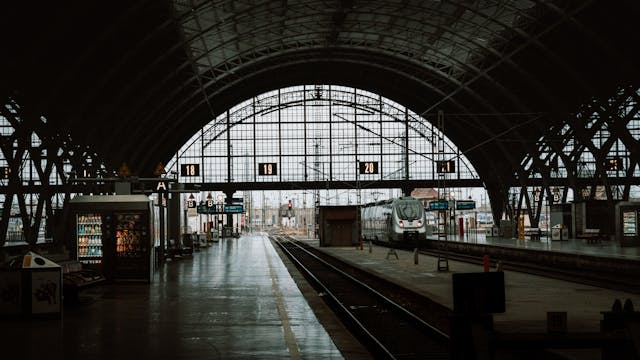
\includegraphics[width = 0.5\textwidth]{image.jpeg}
    \caption{Cool train station}
    \label{fig: image}
\end{figure*}

\end{ZhChapter}
% 章節二 Chapter 2
\begin{ZhChapter}

\chapter{若標題太長,則可以分成兩行排列的形式撰寫}

\section{名詞定義(小標)}

定義定義定義定義定義定義\cite{latex2e},定義定義定義定義,定義定義定義定義定義定義定義定義定義定義,定義定義。

\begin{table*}[htbp]
    \centering
    \caption{表格範例標題} \label{tab: complexity}
    \makebox[\linewidth][c]{
    \renewcommand\arraystretch{1.2}{
        \begin{tabular}{| l | c  c  c  c |}
        \hline
        Protocol & $P$ & $CS_1$ & $CS_2$ & $RG$ \\
        \hline
        MSSMul & $O(1)$, $O(1)$, N/A & $O(n-t)$, $O(n)$, $O(1)$ & $O(n-t)$, $O(n)$, N/A & $O(1)$, $O(n)$, $O(n)$ \\
        SC & $O(1)$, $O(1)$, N/A & $O(n-t)$, $O(n)$, $O(1)$ & $O(n-t)$, $O(n)$, N/A & $O(1)$, $O(n)$, $O(n)$ \\
        \hline 
        \end {tabular}
    }}
\end {table*}

\section{模型說明(小標)}

說明說明說明說明,說明說明說明說明說明說明說明說明說明說明說明說明,說明說明說明說明說明說明說明說明。

\begin{figure*}[htbp]
    \centering
    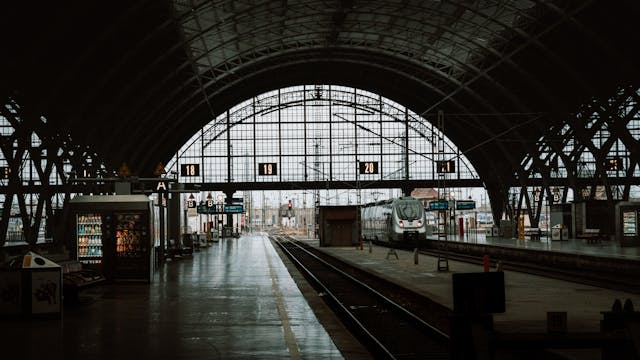
\includegraphics[width = 0.5\textwidth]{image.jpeg}
    \caption{Cool train station}
    \label{fig: image}
\end{figure*}

\end{ZhChapter}
% 新增你自己的章節... Add chapters here

% 參考文獻,請在段落上隨意註解,你同時需要 reference.bib
% Please choose the citation style depending on your academic discipline involved. The most common styles are as follows: APA, IEEE, MLA, Vancouver, etc.
% To avoid personal information leaks, it is recommended not to add “Author Introduction” at the end of the thesis. It is still fine to add ‘Author Introduction' meet the requirement of your department, but make sure to remove any address and phone number information.
\addcontentsline{toc}{chapter}{References}
\printbibliography[title=References]

\end{document}
